\documentclass{article}

\usepackage{graphicx}
\usepackage{tikz}
\usepackage{tikzsymbols}
\usetikzlibrary{calc,patterns,shapes.geometric}
\pagestyle{empty}
\usepackage[margin=0pt]{geometry}
\geometry{papersize={14in,12in}}

\def\centerarc[#1](#2)(#3:#4:#5){\draw[#1] ($(#2)+({#5*cos(#3)},{#5*sin(#3)})$) arc (#3:#4:#5);}

\begin{document}
	\begin{figure}
		\centering
		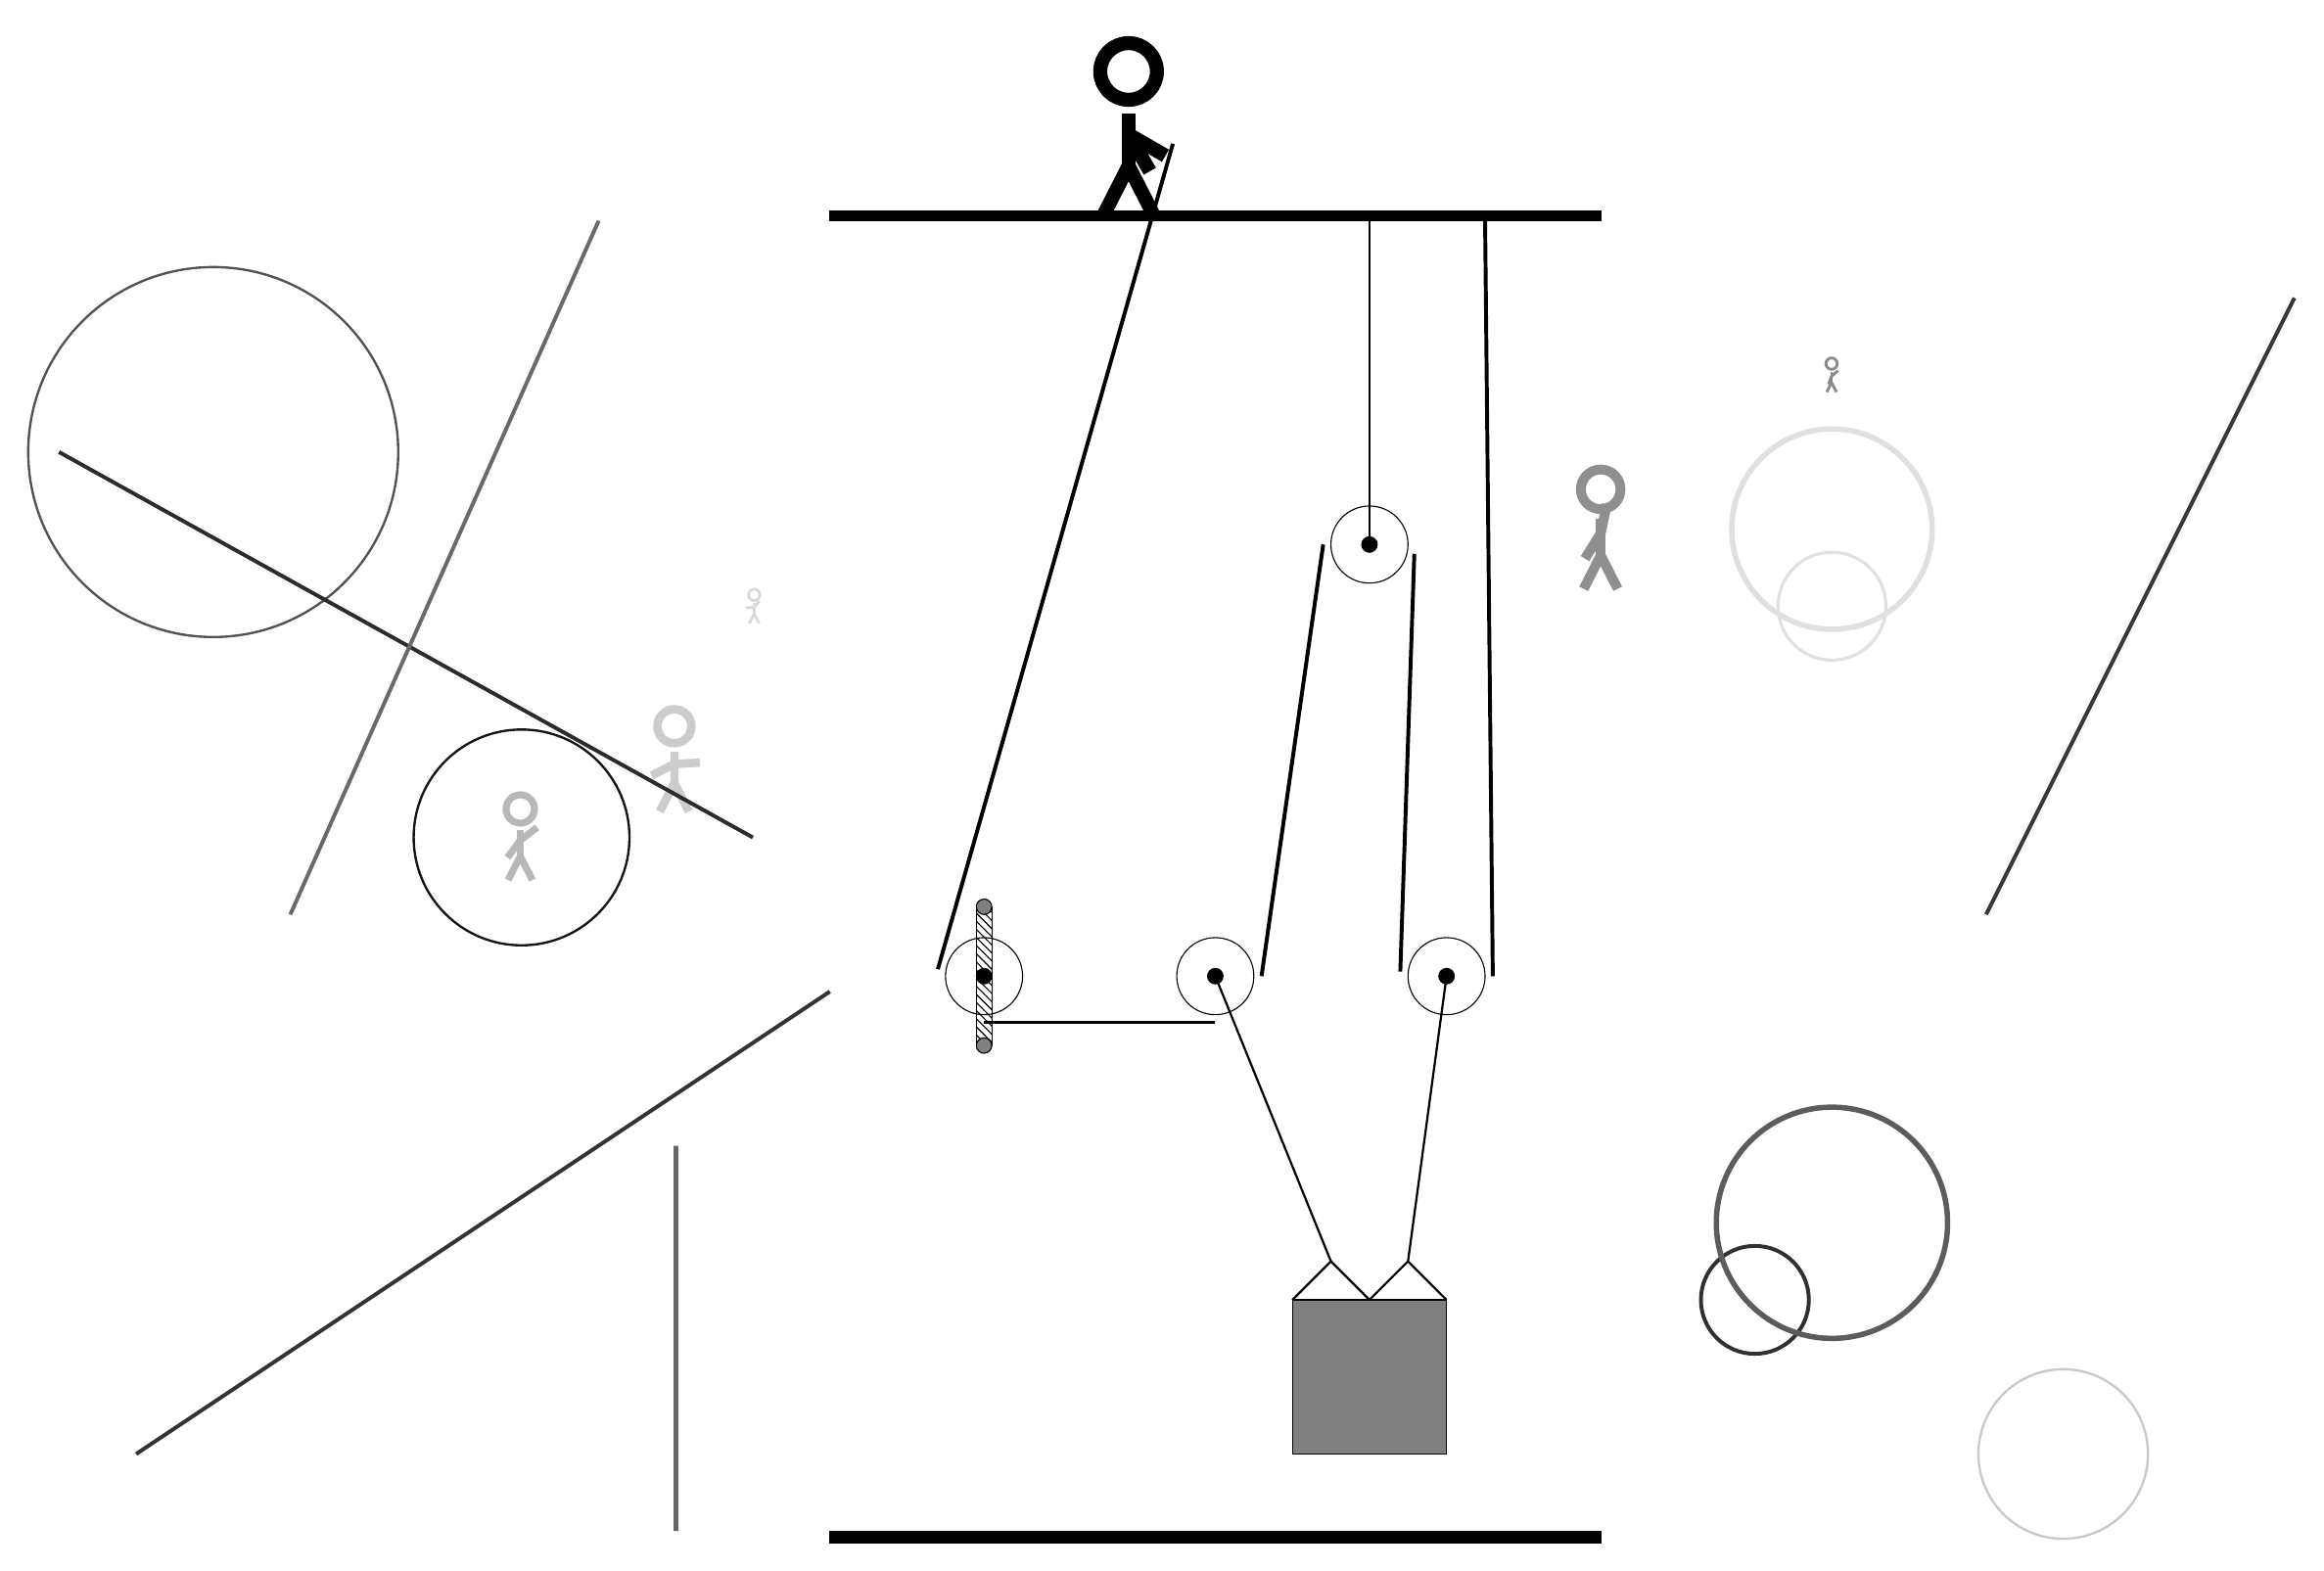
\begin{tikzpicture}
			%%%%% START %%%%%
			
			\draw[fill=black] (-4, 14) rectangle (6, 14.125);
			
			\draw (1, 4.2) circle (0.5);
			\draw[fill=black] (1, 4.2) circle (0.1);
			
			\draw (3, 9.8) circle (0.5);
			\draw[fill=black] (3, 9.8) circle (0.1);
			\draw[thick] (3, 9.8) -- (3, 14);
			
			\draw (4, 4.2) circle (0.5);
			\draw[fill=black] (4, 4.2) circle (0.1);
			
			\node[line width=0.5mm, color=black!20] at (-6, 7) {\Strichmaxerl[6][27][3]};
			
			\draw[line width=0.7mm, color=black!60] (-6, 2) rectangle (-6, -3);
			\draw [line width=0.5mm, color=black!81](8, 0) circle (0.7);
			\draw [line width=0.4mm, color=black!40](13, 6) circle (0.0);
			\draw [line width=0.3mm, color=black!92](-8, 6) circle (1.4);
			\node[line width=0.2mm, color=black!28] at (-8, 6) {\Strichmaxerl[5][53][38]};
			\draw [line width=0.7mm, color=black!64](9, 1) circle (1.5);
			\node[line width=0.4mm, color=black!15] at (-5, 9) {\Strichmaxerl[2][3][52]};
			\draw[line width=0.5mm, color=black!79](11, 5) -- (15, 13);
			\draw [line width=0.4mm, color=black!12](9, 9) circle (0.7);
			\node[line width=0.4mm, color=black!44] at (6, 10) {\Strichmaxerl[7][58][78]};
			\draw [line width=0.7mm, color=black!12](9, 10) circle (1.3);
			\draw [line width=0.3mm, color=black!68](-12, 11) circle (2.4);
			
			\draw[line width=0.5mm, color=black!83](-5, 6) -- (-14, 11);
			\draw [line width=0.3mm, color=black!21](12, -2) circle (1.1);
			\node[line width=0.3mm, color=black!46] at (9, 12) {\Strichmaxerl[2][69][41]};
			
			\draw[line width=0.5mm, color=black!59](-7, 14) -- (-11, 5);
			\draw[line width=0.5mm, color=black!80](-4, 4) -- (-13, -2);
			
			\draw[thick] (4, 4.2) -- (3.5, 0.5);
			\draw[thick] (1, 4.2) -- (2.5, 0.5);
			\draw[thick]  (2, 0) -- (2.5, 0.5) -- (3, 0);
			\draw[thick]  (3, 0) -- (3.5, 0.5) -- (4, 0);
			\draw[fill=black!50] (2, 0) rectangle (4, -2);
			
			\draw (-2, 4.2) circle (0.5);
			\draw[fill=black] (-2, 4.2) circle (0.1);
			\draw[pattern=north west lines, pattern color=black] (-2.1, 5.1) rectangle (-1.9, 3.3);
			\draw[fill=black!50] (-2, 5.1) circle (0.1);
			\draw[fill=black!50] (-2, 3.3) circle (0.1);
			
			\draw[line width=0.5mm] (0.45, 15) -- (-2.6, 4.29);
			\centerarc[line width=0.5mm](-2, 4.2)(160:270:0.6);
			\draw[line width=0.5mm](-2, 3.6) -- (1, 3.6);
			\centerarc[line width=0.5mm](1, 4.2)(270:360:0.6);
			\draw[line width=0.5mm] (1.6, 4.2) -- (2.4, 9.8);
			\centerarc[line width=0.5mm](3, 9.8)(-20:180:0.6);
			\draw[line width=0.5mm](3.582, 9.68) -- (3.4, 4.26);
			\centerarc[line width=0.5mm](4, 4.2)(160:360:0.6);
			\draw[line width=0.5mm](4.6, 4.2) -- (4.5, 14);
			
			\node at (-0.07, 15.2) {\Strichmaxerl[10][120][-30]};
			
			\draw[fill=black] (-4, -3) rectangle (6, -3.15);
			
			%%%%% END %%%%%
		\end{tikzpicture}
	\end{figure}	
\end{document}